\documentclass{beamer}
\title{Git Basics}
\author{David Kouka}
\date{\today}

\usepackage{tikz}
\usetikzlibrary{automata}
\usetikzlibrary{arrows.meta, positioning, calc, shapes.geometric}
\usepackage{graphicx}   % For including images
\usepackage{listings}   % For code listings

\lstset{
    basicstyle=\ttfamily\color{blue}, % Change color and font
    keywordstyle=\color{red},
    commentstyle=\color{green},
    stringstyle=\color{orange},
    columns=flexible,
    keepspaces=true,
    showstringspaces=false,
}

\begin{document}

\frame{\titlepage}

\begin{frame}
    \frame{Table of Contents}
    \tableofcontents
\end{frame}

\section{Version control}
\begin{frame}{Why using version control}
    \begin{itemize}
        \item<1-> Tracking changes \lstinline{git diff} 
\includegraphics[width=0.07\linewidth]{img/register.png}
        \item<2-> Backup and recovery \lstinline{git checkout} 
\includegraphics[width=0.08\linewidth]{img/time_machine.png}

        \item<3-> Collaborative work (authors, conflicts, PR) 
\includegraphics[width=0.07\linewidth]{img/collaborate.png}

        \item<4-> Accountability \lstinline{git blame}
\includegraphics[width=0.09\linewidth]{img/blame.png}

        \item<5-> "Documentation" via commit messages \lstinline{git log}
\includegraphics[width=0.07\linewidth]{img/doc.png}

        \item<6-> Safe experiments \lstinline{git branch} 
\includegraphics[width=0.07\linewidth]{img/experiments.png}

        \item<7-> Easy release management (tags, banches, CI/CD, ...) 
\includegraphics[width=0.07\linewidth]{img/devops.png}

    \end{itemize}
\end{frame}

\section{Hosting}
\begin{frame}{Hosting}
    \only<1-> Git hosting platforms
    \begin{itemize}
        \item<2-> Bitbucket 
\includegraphics[width=0.07\linewidth]{img/logo_bitbucket.png}
        \item<3-> Gitea 
\includegraphics[width=0.07\linewidth]{img/logo_gitea.png}
        \item<4-> Github 
\includegraphics[width=0.07\linewidth]{img/logo_github.png}
        \item<5-> Gitlab 
\includegraphics[width=0.07\linewidth]{img/logo_gitlab.png}
    \end{itemize}
\end{frame}

\section{Cloning}
\begin{frame}{git clone}
    \centering
    \begin{tikzpicture}[
        node distance=2cm,
        image node/.style={inner sep=0, outer sep=0}
    ]
        \only<1>{
            \node[image node] (laptop) {
\includegraphics[width=1.5cm]{img/laptop.png}};
            \node[image node, right=4cm of laptop] (server) {
\includegraphics[width=1.5cm]{img/server.png}};
            \node[image node, below=1cm of server] (potato1_server) {
\includegraphics[width=1cm]{img/potato_1.png}};
        }

        \only<2>{
            \node[image node] (laptop) {
\includegraphics[width=1.5cm]{img/laptop.png}};
            \node[image node, right=4cm of laptop] (server) {
\includegraphics[width=1.5cm]{img/server.png}};
            \node[image node, below=1cm of server] (potato1_server) {
\includegraphics[width=1cm]{img/potato_1.png}};
            \node[image node, below=1cm of laptop] (potato1_laptop) {
\includegraphics[width=1cm]{img/potato_1.png}};
            \draw[->, thick] (potato1_server) -- node[above] {git clone} (potato1_laptop);
        }
    \end{tikzpicture}
\end{frame}

\section{Stage/Commit/Push}
\begin{frame}{Modifications}
    \centering
    
\includegraphics[width=0.5\linewidth]{img/potato_1.png}
\end{frame}
\begin{frame}{Modifications}
    \centering
    
\includegraphics[width=0.5\linewidth]{img/potato_2.png}
\end{frame}

\begin{frame}{git add}
    \centering
    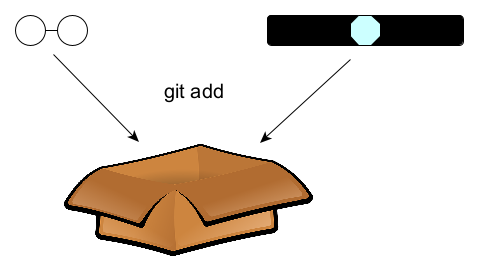
\includegraphics[width=0.5\linewidth]{img/git_add.png}
\end{frame}

\begin{frame}{git commit}
    \centering
    
\includegraphics[width=0.4\linewidth]{img/commit.png}
\end{frame}

\begin{frame}{git push}
    \centering
    \begin{tikzpicture}[
        node distance=2cm,
        image node/.style={inner sep=0, outer sep=0}
    ]
        \only<1>{
            \node[image node] (laptop) {
\includegraphics[width=1.5cm]{img/laptop.png}};
            \node[image node, below=1cm of laptop] (potato2_laptop) {
\includegraphics[width=1cm]{img/potato_2.png}};
            \node[image node, right=4cm of laptop] (server) {
\includegraphics[width=1.5cm]{img/server.png}};
            \node[image node, below=1cm of server] (potato1_server) {
\includegraphics[width=1cm]{img/potato_1.png}};
        }

        \only<2>{
            \node[image node] (laptop) {
\includegraphics[width=1.5cm]{img/laptop.png}};
            \node[image node, right=4cm of laptop] (server) {
\includegraphics[width=1.5cm]{img/server.png}};
            \node[image node, below=1cm of server] (potato2_server) {
\includegraphics[width=1cm]{img/potato_2.png}};
            \node[image node, below=1cm of laptop] (potato2_laptop) {
\includegraphics[width=1cm]{img/potato_2.png}};
            \draw[->, thick] (potato2_laptop) -- node[above] {git push} (potato2_server);
            \node[image node, right=1.4cm of laptop] (delivery) {
\includegraphics[width=1.5cm]{img/delivery.png}};
        }
    \end{tikzpicture}
\end{frame}

\section{Pull}
\begin{frame}{git pull}
    \centering
    \begin{tikzpicture}[
        node distance=2cm,
        image node/.style={inner sep=0, outer sep=0}
    ]

        \only<1>{
            \node[image node] (laptop) {
\includegraphics[width=1.5cm]{img/laptop.png}};
            \node[image node, below=1cm of laptop] (potato2_laptop) {
\includegraphics[width=1cm]{img/potato_2.png}};
            \node[image node, right=2cm of laptop] (server) {
\includegraphics[width=1.5cm]{img/server.png}};
            \node[image node, below=1cm of server] (potato2_server) {
\includegraphics[width=1cm]{img/potato_2.png}};
            \node[image node, right=2cm of server] (laptop2) {
\includegraphics[width=1.5cm]{img/laptop.png}};
            \node[image node, below=1cm of laptop2] (potato1_laptop2) {
\includegraphics[width=1cm]{img/potato_1.png}};
        }
        \only<2>{
            \node[image node] (laptop) {
\includegraphics[width=1.5cm]{img/laptop.png}};
            \node[image node, below=1cm of laptop] (potato2_laptop) {
\includegraphics[width=1cm]{img/potato_2.png}};
            \node[image node, right=2cm of laptop] (server) {
\includegraphics[width=1.5cm]{img/server.png}};
            \node[image node, below=1cm of server] (potato2_server) {
\includegraphics[width=1cm]{img/potato_2.png}};
            \node[image node, right=2cm of server] (laptop2) {
\includegraphics[width=1.5cm]{img/laptop.png}};
            \node[image node, below=1cm of laptop2] (potato2_laptop2) {
\includegraphics[width=1cm]{img/potato_2.png}};
            \draw[->, thick] (potato2_server) -- node[above] {git pull} (potato2_laptop2);
        }
    \end{tikzpicture}
\end{frame}

\section{Branches}
\begin{frame}{git branch}
    \begin{tikzpicture}[
            node/.style={circle, draw=black, very thick, minimum size=15mm},
            img/.style={minimum size=15mm}
        ]

        \node[node] (main) {main};
        \node[img] (img1) [right=of main] {
\includegraphics[width=15mm]{img/bunshin.png}};
        
        \pause

        \node[node] (rasengan) [below left=of main] {\small rasengan};
        \node[img] (img2) [left=of rasengan] {
\includegraphics[width=15mm]{img/bunshin.png}};

        \node[node] (senin) [below right=of main] {senin};
        \node[img] (img3) [right=of senin] {
\includegraphics[width=15mm]{img/bunshin.png}};

        \draw[->] (main) -- (rasengan) node[midway, left] {\texttt{git branch rasengan}};
        \draw[->] (main) -- (senin) node[midway, right] {\texttt{git branch senin}};

    \end{tikzpicture}
\end{frame}

\begin{frame}{git branch}
    \begin{tikzpicture}[
            node/.style={circle, draw=black, very thick, minimum size=15mm},
            img/.style={minimum size=15mm}
        ]

        \node[node] (main) {main};
        \node[img] (img1) [right=of main] {
\includegraphics[width=15mm]{img/bunshin.png}};
        
        \node[node] (rasengan) [below left=of main] {\small rasengan};
        \node[img] (img2) [left=of rasengan] {
\includegraphics[width=15mm]{img/rasengan.png}};

        \node[node] (senin) [below right=of main] {senin};
        \node[img] (img3) [right=of senin] {
\includegraphics[width=15mm]{img/sage.png}};

        \draw[->] (main) -- (rasengan) node[midway, left] {\texttt{git branch rasengan}};
        \draw[->] (main) -- (senin) node[midway, right] {\texttt{git branch senin}};

    \end{tikzpicture}
\end{frame}


\section{Merge}
\begin{frame}{git merge}
    \begin{tikzpicture}[
            node/.style={circle, draw=black, very thick, minimum size=15mm},
            img/.style={minimum size=15mm}
        ]

        \node[node] (main) {main};
        \node[img] (img1) [right=of main] {
\includegraphics[width=15mm]{img/bunshin.png}};
        
        \node[node] (rasengan) [below left=of main] {\small rasengan};
        \node[img] (img2) [left=of rasengan] {\includegraphics[width=15mm]{img/rasengan.png}};
        
        \node[node] (senin) [below right=of main] {senin};
        \node[img] (img3) [right=of senin] {\includegraphics[width=15mm]{img/sage.png}};

        \draw[->] (main) -- (rasengan) node[midway, left] {\texttt{git branch rasengan}};
        \draw[->] (main) -- (senin) node[midway, right] {\texttt{git branch senin}};

        \node[node] (merge) [below=of $(rasengan.south)!0.5!(senin.south)$] {merge};
        \node[img] (img4) [right=of merge] {\includegraphics[width=15mm]{img/naruto_sage_rasengan.png}};
        
        \draw[->] (rasengan) -- (merge) node[midway, left] {\texttt{git merge}};
        \draw[->] (senin) -- (merge) node[midway, right] {\texttt{git merge}};
        
    \end{tikzpicture}
\end{frame}

\section{Conflicts}
\begin{frame}{conflicts}
    \begin{tikzpicture}[
            node/.style={circle, draw=black, very thick, minimum size=5mm},
            img/.style={minimum size=7mm}
        ]
        \node[node] (main) {};
        \pause

        \node[node] (udon_left) [below left=of main] {};
        \node[img] (img1) [left=of udon_left] {\includegraphics[width=7mm]{img/udon.png}};
        \node[node] (udon_right) [below right=of main] {};
        \node[img] (img2) [right=of udon_right] {\includegraphics[width=7mm]{img/udon.png}};
        \draw[->] (main) -- (udon_left) node[midway, left] {};
        \draw[->] (main) -- (udon_right) node[midway, right] {};
        \pause

        \node[node] (eggs_left) [below=of udon_left] {};
        \node[img] (img3) [left=of eggs_left] {\includegraphics[width=7mm]{img/eggs.png}};
        \node[node] (eggs_right) [below=of udon_right] {};
        \node[img] (img4) [right=of eggs_right] {\includegraphics[width=7mm]{img/eggs.png}};
        \draw[->] (udon_left) -- (eggs_left) node[midway, below] {};
        \draw[->] (udon_right) -- (eggs_right) node[midway, below] {};
        \pause

        \node[node, fill=red] (soy_left) [below=of eggs_left] {};
        \node[img] (img5) [left=of soy_left] {\includegraphics[width=7mm]{img/soy_sauce.png}};
        \node[node, fill=blue] (garlic_right) [below=of eggs_right] {};
        \node[img] (img5) [right=of garlic_right] {\includegraphics[width=7mm]{img/garlic.png}};
        \draw[->] (eggs_left) -- (soy_left) node[midway, below] {};
        \draw[->] (eggs_right) -- (garlic_right) node[midway, below] {};
        \pause

        \node[node] (ramen_left) [below=of soy_left] {};
        \node[img] (img5) [left=of ramen_left] {\includegraphics[width=7mm]{img/ramen.png}};
        \node[node] (ramen_right) [below=of garlic_right] {};
        \node[img] (img6) [right=of ramen_right] {\includegraphics[width=7mm]{img/ramen.png}};
        \draw[->] (soy_left) -- (ramen_left) node[midway, below] {};
        \draw[->] (garlic_right) -- (ramen_right) node[midway, below] {};
        \pause

        \node[node, minimum size = 3mm] (merge) [below=of $(ramen_left.south)!0.5!(ramen_right.south)$] {\small x};
        \draw[->] (ramen_left) -- (merge) node[midway, left] {\texttt{???}};
        \draw[->] (ramen_right) -- (merge) node[midway, right] {\texttt{???}};
    \end{tikzpicture}
\end{frame}

\begin{frame}{First commit}
    \begin{tikzpicture}[
            node/.style={circle, draw=black, very thick, minimum size=5mm},
            img/.style={minimum size=7mm}
        ]
        \node[node] (main) {\small main};
        \pause

        \node[node] (udon_left) [below left=of main] {};
        \node[img] (img1) [left=of udon_left] {\includegraphics[width=7mm]{img/udon.png}};
        \draw[->] (main) -- (udon_left) node[midway, left] {};

        \node[node] (eggs_left) [below=of udon_left] {};
        \node[img] (img3) [left=of eggs_left] {\includegraphics[width=7mm]{img/eggs.png}};
        \draw[->] (udon_left) -- (eggs_left) node[midway, below] {};

        \node[node, fill=red] (soy_left) [below=of eggs_left] {};
        \node[img] (img5) [left=of soy_left] {\includegraphics[width=7mm]{img/soy_sauce.png}};
        \draw[->] (eggs_left) -- (soy_left) node[midway, below] {};

        \node[node] (ramen_left) [below=of soy_left] {};
        \node[img] (img5) [left=of ramen_left] {\includegraphics[width=7mm]{img/ramen.png}};
        \draw[->] (soy_left) -- (ramen_left) node[midway, below] {};

        \node[node] (merge) [below right=of ramen_left] {\small main};
        \draw[->] (ramen_left) -- (merge) node[midway, left] {\texttt{git merge}};
    \end{tikzpicture}
\end{frame}

\begin{frame}{2nd commit conflict}
    \begin{tikzpicture}[
            node/.style={circle, draw=black, very thick, minimum size=5mm},
            img/.style={minimum size=7mm}
        ]
        \node[node] (main) {};

        \node[node] (udon_right) [below right=of main] {};
        \node[img] (img2) [right=of udon_right] {\includegraphics[width=7mm]{img/udon.png}};
        \draw[->] (main) -- (udon_right) node[midway, right] {};

        \node[node] (eggs_right) [below=of udon_right] {};
        \node[img] (img4) [right=of eggs_right] {\includegraphics[width=7mm]{img/eggs.png}};
        \draw[->] (udon_right) -- (eggs_right) node[midway, below] {};

        \node[node, fill=blue] (garlic_right) [below=of eggs_right] {};
        \node[img] (img5) [right=of garlic_right] {\includegraphics[width=7mm]{img/garlic.png}};
        \draw[->] (eggs_right) -- (garlic_right) node[midway, below] {};

        \node[node] (ramen_right) [below=of garlic_right] {};
        \node[img] (img6) [right=of ramen_right] {\includegraphics[width=7mm]{img/ramen.png}};
        \draw[->] (garlic_right) -- (ramen_right) node[midway, below] {};

        \node[node, minimum size = 3mm] (merge) [below left=of ramen_right] {\small x};
        \draw[->] (ramen_right) -- (merge) node[midway, right] {\texttt{???}};
    \end{tikzpicture}
\end{frame}

\begin{frame}{Resolving Conflicts}
\centering
    \begin{tikzpicture}[
            node/.style={circle, draw=black, very thick, minimum size=5mm},
            img/.style={minimum size=7mm}
        ]

    \node[node, diamond] (merge) {merge?};
    \pause

    \node[node, below left=of merge, label=below:Incoming, fill=red] (incoming) {};
    \node[img] (img1) [left=of incoming] {\includegraphics[width=1.5cm]{img/soy_sauce.png}};
    \draw[->] (merge) -- (incoming);
    \pause

    \node[node, below=of merge, label=below:Current, fill=blue] (current) {};
    \node[img] (img2) [below=of current] {\includegraphics[width=1.1cm]{img/garlic.png}};
    \draw[->] (merge) -- (current);
    \pause

    \node[node, below right=of merge, label=below:Both, fill=purple] (both) {};
    \node[img] (img3) [right=of both] {\includegraphics[width=1.5cm]{img/soy_sauce.png}};
    \node[img] (img4) [right=of img3] {\includegraphics[width=1.1cm]{img/garlic.png}};
    \draw[->] (merge) -- (both);

\end{tikzpicture}
\end{frame}

\section{Getting further}
\begin{frame}{Getting further}
    \begin{itemize}
        \item<1-> \lstinline{git status}
        \item<2-> submodules
        \item<3-> signed commits
        \item<4-> \href{https://education.github.com/git-cheat-sheet-education.pdf}{Cheat Sheet}
    \end{itemize}
    
\end{frame}

\section{Questions}
\begin{frame}{Questions ?}
    \centering
    \includegraphics[width=0.7\linewidth]{img/naruto_ramen.png}
\end{frame}

\end{document}
